\documentclass[a4paper,12pt]{article}
\usepackage[left=2.5cm,right=2.5cm,top=2.5cm,bottom=2.5cm]{geometry} 
\usepackage{color}
\usepackage[usenames,dvipsnames]{xcolor}
\usepackage{amsmath,amssymb,amsthm,algorithm,algorithmic,graphicx,yhmath,url,enumitem,lscape,mathtools}
\usepackage{wrapfig,subfigure}

\newcounter{problem}
\newenvironment{problem}{\refstepcounter{problem} \noindent {\bf Problem \arabic{problem}}}{\newpage}
\newenvironment{solution}{\vspace{0.3cm} \par \noindent {\bf Solution}}{}
\newenvironment{verification}{\vspace{0.3cm} \par \noindent {\bf Verification}}{}
\newenvironment{hint}{\vspace{0.3cm} \par {\bf Hint:}}{}

\newcounter{remark}
\newenvironment{remark}{\refstepcounter{remark} \vspace{0.3cm} \par \noindent {\bf Remark \arabic{remark}}}{\vspace{0.3cm}}
\newcounter{lesson}
\newenvironment{lesson}{\refstepcounter{lesson} \vspace{0.3cm} \par \noindent {\bf Lesson \arabic{lesson}}}{\vspace{0.3cm}}
\newcommand{\R}{\mathbb{R}}
\newcommand{\N}{\mathbb{N}}
\newcommand{\Rn}{\mathbb{R}^n}
\newcommand{\Rnn}{\mathbb{R}^{n \times n}}
\newcommand{\bes}{\begin{equation*}}
\newcommand{\ees}{\end{equation*}}
\newcommand{\be}{\begin{equation}}
\newcommand{\ee}{\end{equation}}
\newcommand{\eps}{\epsilon}
\newcommand{\fl}{\text{fl}}

\begin{document}

\title{5DV005, Fall 2018, Lab session 3}
\author{Carl Christian Kjelgaard Mikkelsen}

\maketitle
\tableofcontents

\section{The time and the place}
The lab session will take place on
\begin{center}
Wednesday, November 21th, 2018, (kl. 13.00-16.00), Room MA416-426.
\end{center}

\section{The problems}

\begin{problem} \label{BadExp} The function {\tt BadExp} is a very, very bad implementation of the natural exponential function
\be
f(x) = e^x = \sum_{j=0}^\infty \frac{x^j}{j!}
\ee
which has been written by somebody who understands that
\be
f(x) = \underset{n \rightarrow \infty}{\lim} \sum_{j=0}^n \frac{x^j}{j!}
\ee
but has no real appreciation of the difference between real arithmetic and floating point arithmetic!
\begin{enumerate}

\item Explain how the update of the variable {\tt term} is related to the fact that 
  \be
  \frac{x^{j+1}}{(j+1)!} = \left(\frac{x^j}{j!}\right) \frac{x}{j+1}.
  \ee

\item Explain the logic underlying the termination of the {\tt while} loop. Why does it make sense?
  
\item \label{simple:test} Develop a minimal working example {\tt work/BadExpMWE1.m} which uses BadExp to generate a plot similar to Figure \ref{fig:bad_wolf}. Use the points {\tt x = linspace(-30,30,1025)} to sample {\tt BadExp}.
\end{enumerate}

\begin{figure}[ht]
  \centering
  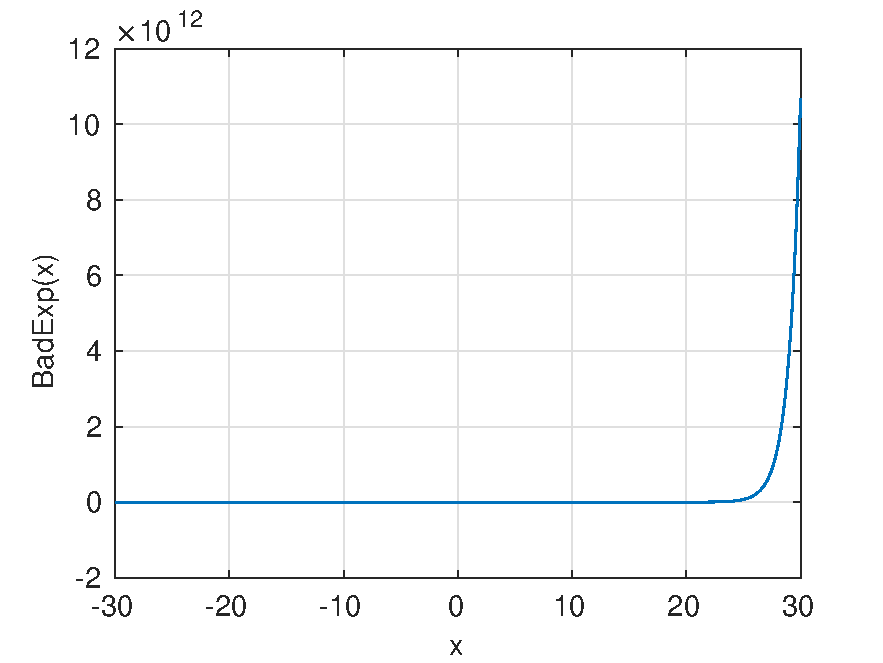
\includegraphics[width=10cm]{BadExp.pdf} \caption{A deceiving plot of the graph of {\tt BadExp}, the bad implementation of the natural exponential function} \label{fig:bad_wolf}
\end{figure}

The graph appears acceptable, but appearances can be quite deceiving! An alarm bell should go off in your head when you notice the extreme range of function values which completely obfuscates any details towards the left end of the plot. Our target $T$ is $T(x) = f(x)$. Our approximation $A$ is $A(x) = \text{{\tt BadExp}}(x)$.

\begin{enumerate}[resume]
  
\item Extend {\tt BadExpMWE1} to generate a second figure which shows the relative error, i.e., the fraction 
\be
R(x) = \frac{T(x) - A(x)}{T(x)}
\ee
Aggressive measures are necessary to get a good impression of the relative error. Apply the {\tt MATLAB} commands {\tt abs} and {\tt log10} as needed. Produce a figure similar to Figure \ref{fig:bad_wolf_relative_error}.

\item Identify the points where the absolute value of the relative error is strictly less than unity.

\item What can be said about the sign of the computed value if the relative error is strictly less than unity?

\begin{figure}[ht]
\centering
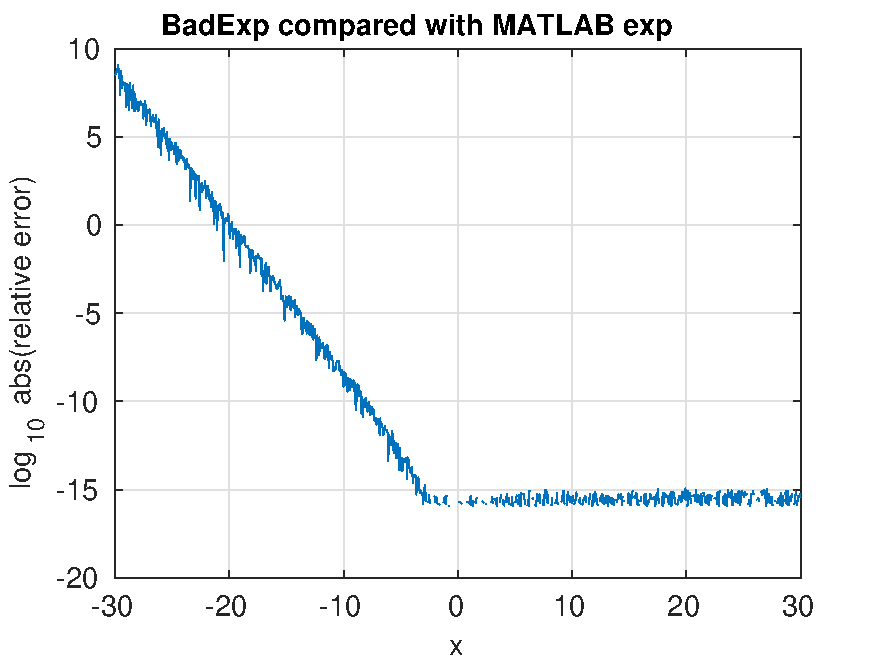
\includegraphics[width=14cm]{BadExpRelErr.pdf} \caption{An illustration of the size of the absolute value of the relative error for {\tt BadExp}. The functions {\tt abs} and {\tt log10} have been applied to allow us to see both very small and very large values of the relative error.} \label{fig:bad_wolf_relative_error}
\end{figure}

\item \label{idx:definition} The real function $x \rightarrow e^{x}$ is always strictly positive, but {\tt BadExp} returns negative values, which is totally unacceptable! Use the {\tt find} and {\tt numel} commands to verify, that exactly 75 of the 1025 values returned by {\tt BadExp} are negative! {\tt idx = find(y<0)} and {\tt x(idx)} are useful commands, right?
  
\item Determine the sign of the entries of {\tt x} for which the corresponding entries of {\tt y} are all negative. The {\tt sign} command can be useful.
\end{enumerate}

\end{problem}

\begin{problem} The problems in {\tt BadExp} are limited to negative values of the input argument! There is nothing wrong with the sign of {\tt BadExp} for positive values and the relative error is rather small here. There is a function called {\tt MyExp} which calls {\tt BadExp}, exploiting the trivial identity
\be \label{exp:identity}
e^x = \frac{1}{e^{-x}},
\ee
in order to avoid working directly with negative values of the argument $x$.

\begin{enumerate}
\item Explain how {\tt GoodExp} isolates the positive and negative input arguments.
\item Explain how {\tt GoodExp} exploits equation \eqref{exp:identity}.
\item Develop a minimal working example {\tt GoodExpMWE1} which is similar to {\tt BadExpMWE1} and generates a plot similar to Figure \ref{fig:good_wolf_relative_error}.
  
\begin{figure}
\centering
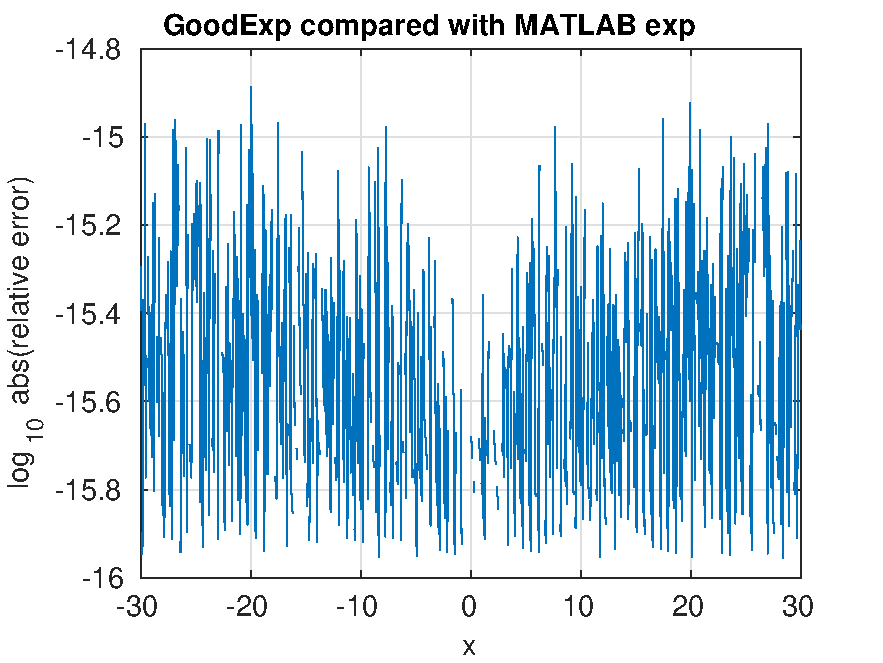
\includegraphics[width=12cm]{GoodExpRelErr.pdf} \caption{A plot of $\log_{10}$ of the absolute value of the relative error for {\tt GoodExp} when compared with the built-in function {\tt exp}.} \label{fig:good_wolf_relative_error}
\end{figure}

\item Verify that absolute value of the relative error is bounded by $12u$ where $u = 2^{-53}$ is the unit round off error in double precision.
  
\item At this point you should be wondering how accurately we can compute $x \rightarrow e^x$ when $x$ is a real number and $x \in [-30,30]$. What are the theoretical limitations? Compute the condition number and show that you can expect the relative error to be around $30u$, where $u$ is the unit round off error. 
\end{enumerate}
\end{problem}

\begin{problem} In this problem you will develop a subroutine which can be used to compute $\sqrt{\alpha}$ for all $\alpha > 0$. Recall that any floating point number $\alpha>0$ can be written as
\be
\alpha = (1.f_1f_2f_3 \dotsc f_k)_2 \times 2^{m}, \quad 
\ee
where $m$ is the exponent and $f_i \in \{0,1\}$ are the individual bits of the mantissa. In IEEE single precision $k=23$. In IEEE double precision $k=52$.

\begin{enumerate} 
\item  Show that in order to compute $\sqrt{\alpha}$ is suffices to have the ability to compute $\sqrt{x}$ where $x \in [1,4]$.
\begin{hint} In general $\sqrt{ab} = \sqrt{a}\sqrt{b}$ and it is very simple to compute the square root of $2^{2k}$, is it not?
\end{hint}
\item  Copy {\tt lab3/scripts/l3p3.m} into {\tt /lab3/work/MySqrt.m} and complete the function according to the specification and the inline comments.
  \begin{remark}
    If your function {\tt MyRoot} (Assignment 1) is ready, then your are encouraged to use it here. Otherwise, you are free to use the more general code {\tt bisection} in the class repository.
  \end{remark}
  
\item Develop a minimal working example {\tt /lab3/work/MySqrt.m} which compares {\tt MySqrt} to the built-in function {\tt sqrt} and generates a figure similar to Figure~\ref{fig:MySqrtRelErr}.

\end{enumerate}

\begin{figure}[ht]
  \centering
  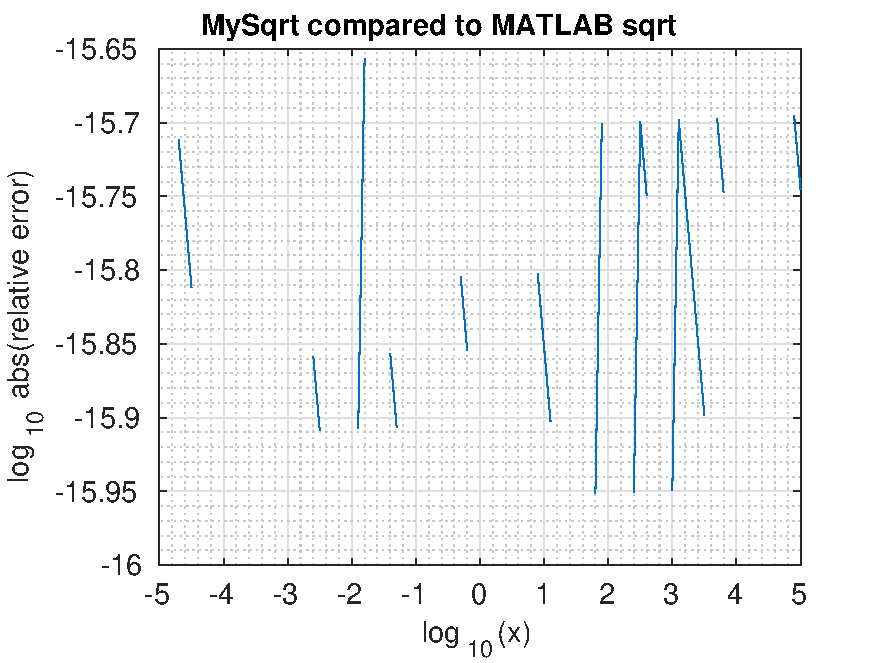
\includegraphics[width=10cm]{MySqrtRelErr.pdf} \caption{Comparison of {\tt MySqrt} to MATLAB's built-in function {\tt sqrt}. } \label{fig:MySqrtRelErr}
\end{figure}


\end{problem}

\begin{problem} This problem develops a function which can compute a standard ballistic table, i.e., the elevation as a function of the range to the target.
  \begin{enumerate}
  \item Copy the function {\tt l3p4.m} into {\tt /work/MyComputeRange} and complete the function according to the specification and the inline comments.
  \item Copy the script {\tt l3p4mwe.m} into {\tt /work/MyComputeRangeMWE1.m} and execute it.
  \item What evidence can you find online to suggest that the computed ballistic table is even remotely related to the real 152 mm D20 howitzer?
  \item Can your program cope with the introduction of a head wind?
  \end{enumerate}

\end{problem}

\bibliographystyle{plain}
  \bibliography{../../../lecture-notes/refs}
  
\end{document}





